%% IEEE TKDE (Transactions on Knowledge and Data Engineering) format
%% Build: latexmk -pdf main_tkde.tex
\documentclass[10pt,journal,compsoc]{IEEEtran}

\usepackage{graphicx}
\usepackage{amsmath}
\usepackage{amssymb}
\usepackage{booktabs}
\usepackage{array}
\usepackage{url}
\usepackage[nocompress]{cite}
\usepackage{enumitem}
\setlist{itemsep=1pt,topsep=3pt,parsep=0pt}
\newcolumntype{P}[1]{>{\raggedright\arraybackslash}p{#1}}
\emergencystretch=3em

% Figures produced separately appear in figures/. The build passes before they exist.
\newcommand{\figseedref}{\IfFileExists{figures/fig_seed_forest_r62.pdf}{, Fig.~\ref{fig:seedforest}}{}}
\newcommand{\figcostref}{\IfFileExists{figures/fig_cost_quality_r64.pdf}{, Fig.~\ref{fig:costquality}}{}}

\begin{document}

\title{What Reaches the Graph Decides Held-Out Question Answering in Knowledge Graph Construction}

\author{Minwoo~Kim,
        Hail~Jung,
        and~Hongdon~Lee% <-this % stops a space
\IEEEcompsocitemizethanks{\IEEEcompsocthanksitem M.~Kim and H.~Lee are with the Manufacturing AX Research Laboratory, INTERX, Seoul 06193, Republic of Korea.\protect\\
E-mail: \{mw.kim, hongdon.lee\}@interxlab.com.
\IEEEcompsocthanksitem H.~Jung is with the Department of Industrial and Systems Engineering, Seoul National University of Science and Technology, Seoul 01811, Republic of Korea, and also with INTERX, Seoul 06193, Republic of Korea.\protect\\
E-mail: hail95@seoultech.ac.kr.
}% <-this % stops an unwanted space
\thanks{Manuscript received Month DD, YYYY; revised Month DD, YYYY.}}

% The paper headers
\markboth{IEEE Transactions on Knowledge and Data Engineering,~Vol.~XX, No.~X, Month~2026}%
{Kim \MakeLowercase{\textit{et al.}}: What Reaches the Graph Decides Held-Out Question Answering}

\IEEEtitleabstractindextext{%
\begin{abstract}
Language models build knowledge graphs from text, but it is unclear which parts of a competency-question (CQ) pipeline make a graph answer unseen questions. We varied the pipeline one component at a time and scored the graphs on held-out questions, on two corpora and two model families, with CQs generated from the corpus text. A relation vocabulary induced from the corpus, without gold knowledge, raised single-pass answer correctness by 16.3 points on the multi-hop corpus and 12.5 on the second, and a vocabulary induced outside the evaluation documents also raised it. With a 22-name relation list, extraction from every chunk without CQs matched the combined pipeline in grounded question answering (QA), at 106k tokens per unit against 838k and with more precise facts. Without any vocabulary, the same extraction scored .558 grounded QA against .430 for iText2KG, .445 for EDC and .213 for AutoSchemaKG, three public extractors. With the list and at equal fact count, the CQ-guided pass scored 39.1 points above a random subset of the listed extraction and held against further selectors. A corpus-induced relation vocabulary with extraction from every chunk is a simple, strong baseline for CQ-driven graph construction. We release plans, code and graphs.
\end{abstract}


\begin{IEEEkeywords}
Competency questions, knowledge graph construction, question answering, relation vocabulary.
\end{IEEEkeywords}}

\maketitle

\IEEEdisplaynontitleabstractindextext
\IEEEpeerreviewmaketitle

\section{Introduction}
\label{sec:intro}

Published competency-question (CQ) driven knowledge-graph pipelines change several components at once and report one final score, so it is unknown which component improves the finished graph's answers to questions it never saw during construction. We varied the components one at a time and found that held-out question answering (QA) follows what reaches the graph. Grounded QA is the share of questions answered correctly with support from retrieved graph facts. A relation list, 22 relation names given to the extractor, raised it by 4.5 to 14.7 points across four pipelines. Seeded extraction (extraction from every chunk without CQs, with the relation list) has grounded QA that was not distinguishable from that of the combined pipeline (95\% interval [$-$3.1, 3.5]; added arm, descriptive). It used 106k tokens per unit against 838k, and the combined pipeline's first pass alone reached .607 at 277k.

Nothing guarantees that a graph an LLM pipeline builds from text can answer the questions people will ask. Ontology engineering approaches this with competency questions~\cite{gruninger1995methodology,noy2001ontology101}. A CQ states something the ontology must answer, so a set of CQs scopes and tests it. In this pipeline a CQ is a question generated from a chunk, with an expected answer span, and the conclusions below are scoped to this CQ pipeline. Recent pipelines generate CQs from text, grow a schema from them, run them against the graph and repair what fails, a cycle we call the repair loop (Section~\ref{sec:related}).

Consider the question ``What is the cause of death of director of film Wedding Bills?'' from 2WikiMultihopQA~\cite{ho2020twowiki}. According to the source text, the director, Erle C. Kenton, died in Glendale ``from Parkinson's disease''. With Qwen, the graph built by a single-pass pipeline with no relation list holds the edge from the film to Kenton but no cause-of-death triple for him. The answerer says ``unknown''. Given a list of 22 relation names that includes ``cause of death'', the same pipeline extracts the triple and answers correctly. CQ count, repair rounds and token budget could do the same, so we varied each alone.

Published CQ-driven pipelines~\cite{feng2024ontologygrounded,kaiser2025hydra,choi2026socratickg} and repair loops~\cite{huang2025tcrqf,chong2026evoontology,zhang2026oak} vary several of these components together, so an arm that reads more text or writes more facts can win without any component helping. Prior schema-guided and schema-inducing extraction shows that a schema helps extraction~\cite{sainz2024gollie,bai2026autoschemakg}, but they vary the schema, not the relation vocabulary of a CQ pipeline at equal volume.

We ran seven experiments and one error analysis (Table~\ref{tab:experiments}) on two corpora and two model families, Qwen and Gemma. Most contrasts use Qwen on 2WikiMultihopQA, and Gemma repeated some. Four pipelines recur: the single pass (L0), the loop (LOOP), extraction without CQs or a schema (U-ext) and our combined pipeline, all defined in Table~\ref{tab:arms} (Section~\ref{sec:pipeline}). Answer correctness drops the support requirement of grounded QA, and code scores both against gold (Section~\ref{sec:design}). Held-out questions stay out of every construction stage, and arms use the same tokens, patch size or fact count wherever volume could confound the comparison. We registered the plans, with hypotheses and decision rules, before the main runs (labels in Section~\ref{sec:design}).

We report three results, each with its status. Registered tests did not find guided repair above random patches of the same size (upper bound 3.1 points against a margin of 5), while the relation list raised every pipeline.
\begin{enumerate}
  \item A relation vocabulary lifts the single pass, and an induced one needs no gold knowledge. A list induced from corpus chunks without gold raised answer correctness on 2WikiMultihopQA by 16.3 points [11.6, 20.2] and on T-REx by 12.5 (both registered), and the effect replicates with Gemma (descriptive; Section~\ref{sec:res-schema}). A T-REx list induced only from passages outside the evaluation shards raised the single pass's grounded QA by 7.4 points over no list (registered). A 2Wiki list induced only outside the evaluation shards also raised the single pass (registered).
  \item With the relation list, extraction from every chunk without CQs was not distinguishable from the combined pipeline in grounded QA (0.3 points below) at a fraction of the tokens, with more precise facts (added arm; precision registered). On answer correctness seeded extraction was 2.3 points higher ([$-$0.2, 4.4], post hoc). On T-REx seeded extraction led by 5.0 points (registered interval). Three public extractors, which received no relation list and ran released defaults, scored 15.8 to 39.2 points below seeded extraction in grounded QA (descriptive; Section~\ref{sec:res-cost}). The graph also answered more questions correctly than retrieval over the same chunks (registered).
  \item With the relation list and an equal fact count, CQ-guided facts scored higher than selections made without CQs. The guided single pass scored 39.1 points above a random subset of seeded extraction on the multi-hop corpus (a registered test asked whether the random subset scores higher; it did not), and the lead held on T-REx and against heuristic, chain-preserving, model-scored, CQ-based and chunk-balanced selections of the same graph (registered). Without the list, the relation-frequency selection scored 8.0 points above the guided pass (registered), and on T-REx the contrast with a random subset was not established.
\end{enumerate}
We release plans, deviation logs, code and graphs.

\section{Related Work}
\label{sec:related}

\paragraph{Competency questions and LLM-assisted ontology engineering.}
Competency questions fix the scope of an ontology before it is built~\cite{gruninger1995methodology,noy2001ontology101}. LLM tools now elicit CQs (OntoChat~\cite{zhang2024ontochat}), draft OWL ontologies from CQs (Ontogenia~\cite{lippolis2025ontogenia}) and verify CQs against an ontology (OE-Assist~\cite{lippolis2025oeassist}). IDEA2 keeps an expert in the loop~\cite{watkissleek2026idea2}.

\paragraph{From CQs to knowledge graphs.}
Feng et al.\ derive relations from CQs and ground graph construction in the resulting ontology~\cite{feng2024ontologygrounded}. HyDRA builds an ontology from CQs that agents agree on~\cite{kaiser2025hydra}, and SocraticKG expands each passage into question--answer pairs before extraction~\cite{choi2026socratickg}.

\paragraph{Iterative repair and prompt optimisation.}
TCR-QF, EvoOntology and OaK repair a graph or an ontology over several rounds~\cite{huang2025tcrqf,chong2026evoontology,zhang2026oak}. A controlled study of ontology generation from insurance contracts found no gain from iterative repair in a single-agent baseline~\cite{talukder2026multiagent}. DSPy, MIPROv2 and GEPA optimise prompts against a metric~\cite{khattab2023dspy,opsahlong2024mipro,agrawal2025gepa} and have been applied to triple extraction and ontology learning~\cite{mihindukulasooriya2025apo,mai2026apolo}.

\paragraph{Text-to-KG extraction and KG-augmented QA.}
iText2KG builds graphs incrementally without a fixed schema~\cite{lairgi2024itext2kg}, and we compare it with our extraction in the same setup (Section~\ref{sec:res-cost}). KGGen~\cite{mo2025kggen} measures extraction, Text2KGBench scores extraction when the ontology is given~\cite{mihindukulasooriya2023text2kgbench}, and GraphRAG combines an entity graph with community summaries for retrieval~\cite{edge2024graphrag}.

\paragraph{Schema-guided extraction, schema induction and QA-based evaluation.}
CodeKGC encodes a pre-defined entity and relation schema in code prompts~\cite{bi2024codekgc}. KnowCoder represents schemas, among them 876 relation types, as code classes that the model follows~\cite{li2024knowcoder}, and GoLLIE reports that label definitions and guidelines in the schema are central to zero-shot extraction~\cite{sainz2024gollie}. EDC (Extract, Define, Canonicalize) runs with a pre-defined target schema or one it induces and canonicalises itself~\cite{zhang2024edc}, and we score that self-induced mode in our setup (Section~\ref{sec:res-cost}). AutoSchemaKG induces a schema from text and reports multi-hop QA gains~\cite{bai2026autoschemakg}; we score it in our setup as well (Section~\ref{sec:res-cost}). HippoRAG scores a schemaless OpenIE graph by multi-hop QA~\cite{gutierrez2024hipporag}. These studies show that a supplied or induced schema steers extraction~\cite{sainz2024gollie,li2024knowcoder,zhang2024edc,bai2026autoschemakg}. Within one pipeline at equal volume we separate the relation vocabulary from the competency-question machinery. A vocabulary induced from the corpus without gold carries the gain on two corpora. With a relation list, extraction without competency questions is not distinguishable from the combined pipeline's grounded question answering and uses fewer tokens (Section~\ref{sec:res-cost}).

\section{Pipeline and Experimental Design}
\label{sec:pipeline-design}
\subsection{The Curation Pipeline and Its Components}
\label{sec:pipeline}

All experiments use one pipeline family, which reads a corpus split into chunks and produces a Web Ontology Language (OWL) style schema (TBox) and a set of facts (ABox) stored as Resource Description Framework (RDF) triples. Formally, a constructed knowledge graph is represented as $G = (V, E)$, where $V$ denotes the set of entity vertices and $E \subseteq V \times \mathcal{R} \times V$ denotes directed relational edges labeled by predicates from a relation vocabulary $\mathcal{R}$. Figure~\ref{fig:pipeline} shows the five stages, and Table~\ref{tab:experiments} lists the studies, Exp1 to Exp8.

\begin{figure*}[t]
\centering
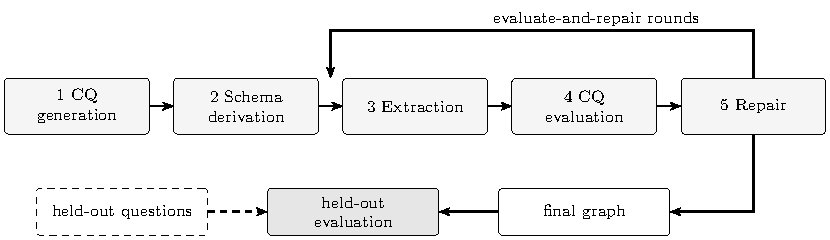
\includegraphics[width=\textwidth]{fig_pipeline.pdf}
\caption{The pipeline builds the graph in five stages, and evaluate-and-repair rounds loop from repair back to schema derivation and extraction. Held-out questions reach only the evaluation of the final graph.}
\label{fig:pipeline}
\end{figure*}

\paragraph{Stages.}
\begin{enumerate}
  \item \emph{CQ generation.} The generator reads a batch of chunks and writes questions that a reader of those chunks should be able to answer. Each CQ, a question generated from a chunk, keeps its source chunk and an expected answer span, which code checks against the chunk.
  \item \emph{Schema derivation.} Classes and properties are derived from the CQs.
  \item \emph{Extraction.} Facts are extracted chunk by chunk, guided by the current schema. Every fact keeps the chunk it came from.
  \item \emph{CQ evaluation.} Each CQ is translated to SPARQL Protocol and RDF Query Language (SPARQL) queries and run against the graph. A deterministic rule first checks that the expected span appears in the result rows. An LLM judge then grades the answer 0, 1 or 2.
  \item \emph{Repair.} Failed CQs are attributed either to the query or to the graph. Graph-side failures produce patches (added facts, merged entities, corrected values or new properties). A gate scores each patch on a reserved set of curation CQs, never on held-out questions, and accepts or rejects it.
\end{enumerate}

\paragraph{Components under test.}
Every study except the Exp6 error analysis changes one of the following components or removes one from the combined pipeline.
\begin{description}
  \item[Relation list.] A relation list from the training split: the 22 most frequent relation types (share of at least 0.1\%) in the evidence inventory of the 2WikiMultihopQA training split, where no evaluation question was used. The names cover the relations of 98.4\% of the 1,216 gold evidence items of the evaluation set. Only the names are given, in alphabetical order, with no frequencies or examples. The names enter the prompts as one block with the same wording and position in every arm with the list (Table~\ref{tab:arms}), and Appendix~\ref{app:seednames} lists them.
  \item[CQ coverage.] Coverage is the share of chunks that are the source of at least one CQ. A first round writes a fixed number of CQs (40 in most experiments). \emph{Expansion} adds CQs over several rounds, each time drawing from chunks that are not yet the source of any CQ, until every chunk is covered.
  \item[CQ count.] Exp8 varies the number of CQs at a fixed or increased token budget.
  \item[Evaluate-and-repair rounds.] Stages 4 and 5 run for several rounds. The loop used in Exp5, and as the LOOP baseline in Exp7, repairs queries first and patches only graph-side failures.
  \item[Budget and extraction passes.] The total number of tokens, and how the remainder is spent. In the combined pipeline, tokens left after expansion go to additional full-corpus extraction passes that ask for facts missing from the current graph.
\end{description}

\paragraph{Where the 22 names come from.}
The original list is the set of relation types with a share of at least 0.1\% in the evidence inventory of the training split, which gives 22 names. An induced list uses no question and no gold relation. The extraction model reads 300 randomly sampled passages (title and first 1,200 characters) in 20 batches of 15 and proposes up to 15 relation names per batch, and the names are normalised to one to four lowercase words. The 80 names proposed in the most batches go to one model call that merges near-duplicates and keeps exactly 22. Induced lists have 22 names so that they equal the size of the original list and differ only in content (Appendix~\ref{app:seednames}).

Table~\ref{tab:arms} defines every arm. The \emph{combined pipeline} (``Combined'' in tables) starts from the relation list, and a \emph{+vocab} suffix on any other arm name means the same pipeline run with that list.

\begin{table*}[t]
\centering
\small\setlength{\tabcolsep}{3.5pt}
\caption{The arms compared. ``Reads and writes'' gives what each arm takes in and produces; the last column gives where the relation list enters the prompts when the arm runs with it.}
\label{tab:arms}
\begin{tabular}{lP{6.2cm}cP{4.6cm}}
\toprule
Arm & Reads and writes & CQs & Where the list enters \\
\midrule
L0 (single pass) & Chunks $\rightarrow$ 40 CQs $\rightarrow$ schema of at most 36 properties $\rightarrow$ facts extracted from every chunk & yes & CQ generation and schema derivation \\
G (Exp4, Exp5) & L0 with the CQ set expanded until every chunk is a CQ source & yes & as L0 \\
GR (Exp4, Exp5) & G plus evaluate-and-repair rounds & yes & as L0 \\
LOOP & L0, then three rounds of CQ evaluation and repair with 20 new CQs per round & yes & CQ generation, schema extension and schema patches \\
Combined & Relation list, CQs expanded to every chunk, an incremental schema with deterministic de-duplication, and extra extraction passes up to the token total of LOOP+vocab on the same unit; CQ evaluation only as an acceptance test, no repair step. ``First pass only'' stops after the first full extraction pass & yes & CQ generation, schema derivation and schema extension \\
U-ext (extraction without CQs) & No CQs and no schema: free-form predicates from every chunk, one call per chunk; the schema is derived afterwards & no & Extraction prompt, after the chunk text and before the instruction (U-ext+vocab) \\
+vocab & Any arm above run with the 22-name relation list (L0+vocab, LOOP+vocab, and U-ext+vocab, called \emph{seeded extraction}; ``Combined'' always has it unless marked no list) & as arm & as in the arm's row \\
L0+vocab$K$ & L0 given $K$ of the 22 names ($K$ = 6, 11, 17; nested random subsets) & yes & CQ generation and schema derivation \\
iText2KG, EDC, AutoSchemaKG & Chunks $\rightarrow$ facts with each public extractor's released defaults and no relation list (EDC also once with the list, Section~\ref{sec:res-cost}); EDC and AutoSchemaKG induce and canonicalise their own schema, and AutoSchemaKG's entity-relation triples are scored & no & none \\
\bottomrule
\end{tabular}
\end{table*}

\subsection{Experimental Design}
\label{sec:design}

\paragraph{Data.}
Dataset questions are held out from every stage of construction and only score the final graph. No loop, gate or prompt sees them. The pipeline generates and uses its own curation CQs freely.

The main corpus is 2WikiMultihopQA (2Wiki)~\cite{ho2020twowiki}. A \emph{shard} is a group of questions together with the union of their context paragraphs, with 8 questions in Exp4 and 16 in Exp5, Exp7 and Exp8. From Exp4 on, each 2Wiki experiment excludes the questions used in the earlier experiments. The second corpus is a movie-domain subset of T-REx~\cite{elsahar2018trex} with 482 documents and 14 relation types, of which 386 documents and 507 questions are held out for evaluation. Exp1 uses a bank of building-ontology questions and appears only in Appendix~\ref{app:experiments}. Exp7 holds 480 held-out questions in 30 shards and two run seeds, with no failed cells. On T-REx, the Exp7 arms use Qwen on 33 held-out shards with one-hop gold. Two lists were used there: the T-REx arms of the Exp7 comparisons (Table~\ref{tab:newchecks}, Fig.~\ref{fig:costquality}) used the 2Wiki relation names, and the arms of Table~\ref{tab:trexseed} used the list induced from the T-REx corpus. The 2Wiki checks and Table~\ref{tab:trexseed} use two run seeds; the T-REx Exp7 arms and the AutoSchemaKG arm use one.

\begin{table*}[t]
\centering
\small\setlength{\tabcolsep}{3.5pt}
\caption{The eight studies (Exp6 is an error analysis, the others each vary one component), the Gemma replication and a third model. Each has a plan, a deviation log, code and results in the released archive.}
\label{tab:experiments}
\begin{tabular}{lp{5.7cm}p{5.0cm}l}
\toprule
 & Question & Data & Models \\
\midrule
Exp1 & Does iterative CQ refinement improve a graph? & Building ontology bank, 35 test questions & Qwen \\
Exp2 & Does iteration improve on one batch of the same CQs? & 2Wiki, 24 shards & Qwen \\
Exp3 & Does prompt optimisation improve on a relation list? & 2Wiki, 400 test questions & Qwen \\
Exp4 & Does a CQ $\rightarrow$ SPARQL $\rightarrow$ judge $\rightarrow$ patch loop help? & 2Wiki, 40 shards & Qwen \\
Exp5 & Does a loop with query repair and a rejecting gate help? & 2Wiki, 24 shards $\times$ 2 run seeds & Qwen \\
Exp6 & Which error types occur, and can Shapes Constraint Language (SHACL) see them? & Exp2 graphs & --- \\
Exp7 & What do the combined pipeline's parts add? & 2Wiki, 30 shards $\times$ 2 run seeds & Qwen \\
Exp8 & How do CQ count, budget and hybrid QA interact? & 2Wiki and T-REx, 20 to 33 shards & Qwen, Gemma \\
Replication & Gemma (Exp1, Exp4, Exp5, Exp7, and Exp7's design on T-REx); Exp2 and Exp3 were not repeated & as above & Gemma \\
Third model & Nemotron (Exp5, Exp7 and T-REx; Appendix Table~\ref{tab:replication}) & as above & Nemotron \\
\bottomrule
\end{tabular}
\end{table*}

\paragraph{Exp8 arms.}
The reference arm uses 40 CQs at the 1$\times$ token budget. For each shard the budget comes from a reference run, and an arm stops after using 95\% of it. Other arms are named by CQ count and budget: 160 CQs at 1$\times$, 160 CQs at 4$\times$ and 40 CQs at 4$\times$. The source check is on in the 40-CQ and 160-CQ arms. Each generated CQ is embedded with Qwen3-Embedding-0.6B and compared with the top 5 retrieved chunks, and a CQ that fails is regenerated up to 3 times.

\paragraph{Metrics.}
Evidence recall and all QA measures are scored by code against gold. An LLM judge is used in three places. The builder's own model family (Qwen3.8-Flash-Next) judges the pipeline's internal CQ evaluation (stage 4) and the pass rate of fresh CQs, and a model from the other family judges precision in Exp8. Gemma judges Qwen graphs and Qwen judges Gemma graphs, and the CQ checks use the builder's family.
\begin{itemize}
  \item \emph{Evidence recall} is the share of gold evidence triples present in the graph. A triple counts as present when a chunk-cited triple links the same entity pair under a predicate of the same relation class. \emph{Uncapped recall} counts every such triple. \emph{Capped recall} is recall under a per-question triple budget: the budget is two triples for every source sentence of the question's paragraphs, and each gold evidence counts the probability that a uniform random subset of that question's graph slice no larger than the budget still holds a matching triple, computed exactly as a hypergeometric expectation without sampling, so padding the graph lowers recall. ``Token budget'' always refers to tokens.
  \item \emph{Answer correctness} is scored by code against the gold answer without the grounding requirement: normalised exact match against the gold answer and its aliases or demonyms, the first token for yes/no questions, exact match for dates, and ``unknown'' counts as wrong.
  \item \emph{Grounded QA} asks a model to answer each held-out question from facts retrieved from the graph. Given an input query $q$ and graph $G$, let $R(q, G) \subseteq G$ denote the retrieved supporting fact subgraph. The grounded correctness indicator $\mathbb{I}_{\text{gc}}(q) \in \{0, 1\}$ evaluates whether the answer generated from $R(q, G)$ is correct and grounded in the retrieved facts. Grounded QA over a set $Q$ of held-out questions is $\frac{1}{|Q|}\sum_{q \in Q} \mathbb{I}_{\text{gc}}(q)$. For comparison questions every gold evidence pair (subject and object, in either direction) must appear in a retrieved fact that cites a chunk containing the evidence. For open questions the gold answer must appear as the subject or object of a retrieved fact. The relation name plays no part in grounded QA; relation classes enter only evidence recall (class-aligned recall). QA-time retrieval is the same for every arm and does not use the list: the question is linked to entity labels (with aliases) by exact n-gram matching, the graph is followed for up to two hops, each entity contributes at most 25 facts ranked by BM25, and the facts in $R(q, G)$ are ordered by hop, then BM25, and capped at 60.
  \item The \emph{pass rate of fresh CQs} (Exp7) uses 40 new CQs per shard and run seed. They are written from 40 random chunks with a neutral prompt and no relation list, and no loop uses them.
  \item For each final graph, SPARQL is generated three times for each fresh CQ. A query passes when it returns at most 20 rows, the expected answer span is among them and the judge scores it 2. The pass rate is the mean over the three generations. 
  \item In Exp8, KG-only QA gives the answerer graph facts only. Hybrid QA gives it up to 30 graph facts (main run; a rerun used up to 60) and the top 3 retrieved passages, and \emph{vector QA} gives it the top 5 passages. Measure F2 takes the vector answer unless it abstains, and then the KG-only answer.
  \item \emph{Precision} is judged on 40 sampled facts per graph by the cross-family judge. Gold evidence covers only the facts that questions need, so unaligned triples are not counted as errors. In the fact precision check on the Exp7 graphs, Gemma judges Qwen facts in one pass.
\end{itemize}

\paragraph{Models.}
We implemented this family of CQ-driven methods as one pipeline. Construction, querying and QA use Qwen3.8-Flash-Next (NVFP4 weights) in Exp1--Exp7, and the Gemma replication repeats the experiments named in Table~\ref{tab:experiments} with Gemma-4-26B-A4B-it. NVIDIA Nemotron-3.5-Lightning-30B-A3B, a third model, ran Exp5, Exp7 and T-REx; its graphs stayed at or below .047 grounded QA in every arm, so model comparisons rest on Qwen and Gemma. Exp8 runs Gemma-4-26B-A4B-it and Qwen3.8-Flash-Next on both corpora. All models were served with vLLM, and Qwen ran with thinking off. The QA answerer decodes at temperature 0 (120 output tokens) and extraction at temperature 0 (1,500 output tokens). First-round CQ generation uses temperature 0.7, later CQ steps use 0, and the judges use 0.

\paragraph{External extractors.}
As an external reference, iText2KG 1.1.0 ran with its default settings on each chunk of the Exp7 2Wiki shards with Qwen. It takes no relation list, so none was given, and the Exp7 answerer and scorer scored its graphs. The public extractor EDC~\cite{zhang2024edc} ran on the same chunks, model and engine with its released defaults (Self Canonicalization). It induces and canonicalises its own schema, so it took no list. A third public extractor, AutoSchemaKG~\cite{bai2026autoschemakg}, ran with its released defaults on the same chunks, model family, answerer and scorer, on 30 shards with one run seed; it also took no list.

\paragraph{Registration and statistics.}
Each experiment has a plan, fixed before the main run, that states hypotheses and decision rules; the labels, the checks added later and the run records are in Appendix~\ref{app:registration}. Status labels follow the plan: \emph{registered} hypotheses were fixed beforehand, \emph{secondary} measures are reported beside them, \emph{descriptive} contrasts report intervals only, and \emph{post hoc} analyses and \emph{added arms} came after the results or after the plan was frozen. The unit of analysis is the shard in Exp2, Exp4, Exp5, Exp7 and Exp8 and the question in Exp1 and Exp3; within a shard we average values over run seeds and compare arms pairwise. Intervals are two-sided 95\% bias-corrected and accelerated (BCa) bootstrap intervals that resample by shard, with 10,000 resamples in Exp7 and Exp8. Primary hypotheses are Holm-corrected within the registered primary family of each plan. Tables give the number of shards as $n$ and state units where both appear (30 shards are 60 shard $\times$ run seed units).

\paragraph{Chunk retrieval.}
On the same 2Wiki units of Exp7, two arms answer from the top 5 chunks retrieved by embedding. Top 5 matches the graph arm's prompt length (791 against 794 tokens, median); one arm also receives the 22-name list as a hint. Answer correctness is the measure, since grounding is defined on graph facts.


\paragraph{Controls for volume.}
Tokens per unit count the construction of an arm and its own CQ evaluation: extraction, CQ generation, the pipeline's SPARQL and judge calls and repair, with retries counted and cached calls billed at their nominal cost. They exclude the held-out QA that scores the graph. The construction of an induced list is a separate step and is not included.
Most comparisons hold volume fixed in one of three ways. Arms with equal token budgets stop at the same share of a reference budget (Exp7, Exp8), and the combined pipeline's budget was the token total of LOOP with the list on the same unit. Its arm without the list used the same budget (837,655 and 838,162 tokens). Exp4 and Exp5 compare evaluation-guided patches with random patches of the same size. In Exp7 we also match fact counts. The check at equal fact count draws a uniform random subset of the facts in each stored U-ext graph, with and without the list. The subset matches the fact count $|E|$ of the corresponding L0 graph, and the same answerer and scorer score it. Its plan was fixed before any model call. Two selections reduced the same graphs to the same fact count. One keeps the facts whose relation is most frequent, the other the facts whose end entities are most central. Both read only the facts already in the graph. A chain-preserving and a model selector read no questions, gold or CQs either and keep exactly the guided pass's fact count: the first keeps the facts that add the most connected two-hop entity paths, and the second has the answer model score each fact's informativeness from its source chunk alone. Two more selectors, over the same stored graph and fact count, read no questions and no gold either: a selection by the CQs (BM25 between each fact and the 40 CQs that the guided pass generated for that unit; top facts kept) and a chunk-balanced selection (facts taken round-robin by chunk, ties by hash).

\section{Relation Vocabulary Raises Held-Out QA}
\label{sec:res-schema}

The relation list raised held-out grounded QA in all four Exp7 pipelines of Qwen on 2Wiki (Table~\ref{tab:exp8}\figseedref). L0 gained 14.7 points ([10.9, 18.4]), LOOP 9.4, the combined pipeline 9.3 and U-ext 4.5, a range of 4.5 to 14.7. The arms are defined in Table~\ref{tab:arms}. In Gemma on 2Wiki the list raised grounded QA over no list by 7.4 points in L0 ([3.3, 11.3]) and 7.5 in LOOP ([1.3, 15.0]). The Gemma combined pipeline gained 9.3 ([5.7, 12.9]). Further contrasts with their status are in Appendix Table~\ref{tab:glance}.

\IfFileExists{figures/fig_seed_forest_r62.pdf}{%
\begin{figure}[t]
\centering
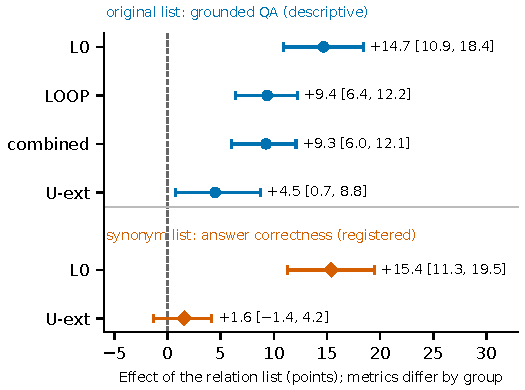
\includegraphics[width=\columnwidth]{figures/fig_seed_forest_r62.pdf}
\caption{The relation list raised held-out grounded QA in all four pipelines, and synonym names raised answer correctness in L0. Differences in points with 95\% intervals, Qwen on 2Wiki. The two groups use different metrics. Top, original list: grounded QA, descriptive. Bottom, synonym list: answer correctness, registered; L0 +15.4 [11.3, 19.5], U-ext +1.6 [$-$1.4, 4.2].}
\label{fig:seedforest}
\end{figure}}{}

Synonym names kept the benefit in L0. No question ID or normalised question text of the list's training split appears among the evaluation questions. No synonym shares a word stem with its original name. In L0 answer correctness rose by 15.4 points (Qwen, 2WikiMultihopQA; [11.3, 19.5], Holm $p$ = 0.0002; Table~\ref{tab:synseed}), and grounded QA rose by 15.8 ([11.5, 20.3]). In U-ext, which already extracts from every chunk, the gain was +1.6 ([$-$1.4, 4.2]), in line with the smaller effect of the original list there (Appendix Table~\ref{tab:seedalign}).

In L0 the synonym list's answer correctness was within 1.7 points of the original list's ([$-$2.0, 5.0]), while the original list gained 13.8 over no list in the stored runs.

A list induced from the corpus, with no gold relations, raised L0 answer correctness by 16.3 points ([11.6, 20.2], Holm $p$ = 0.001, registered). The original list rerun on the same instance gave +15.1 ([10.5, 19.5]); the same arm differed between serving instances (no list .433 stored, .417 rerun), so contrasts are taken within one instance where possible.

The same induction on T-REx, from 300 of that corpus's 386 documents, gave a list of 22 names. No question and no gold relation was used. There it raised the single pass by 13.3 points of grounded QA ([8.0, 23.1], registered: improved) and by 12.5 points of answer correctness (registered: improved, Table~\ref{tab:trexseed}).

A second T-REx list, induced from 96 passages outside the evaluation shards with the same procedure and no question, shares 15 of its 22 names with the first and 6 with the 2Wiki list. With this outside-shard list, the single pass scored 7.4 points above no list in grounded QA ([3.9, 11.4], registered: improved, Holm $p$ = 0.0001; Table~\ref{tab:trexseed}), the same pattern as the first T-REx list.

A second 2Wiki list, induced with the same procedure from 300 of 6,136 chunks outside the evaluation shards and no question, shares 18 of its 22 names with the first induced list and 5 with the training-split list. With it, the single pass scored 15.8 points above no list in grounded QA ([9.6, 21.9], registered: improved, Holm $p$ = 0.0002; Table~\ref{tab:seednames}). Extraction from every chunk gained +3.1 [0.0, 6.5] in grounded QA (registered: improved at the boundary; answer correctness +1.7 [$-$1.0, 4.2], not established).

Answer correctness in L0 depended on how much of the list was given (Table~\ref{tab:seeddose}; reruns on one serving instance). The curve is not monotone. In the nested draw of names used here, 11 of the 22 names scored 10.5 points above no list ([5.5, 14.5]); each partial setting (6, 11 and 17 names) is a single draw of names (post hoc, descriptive). The dip at 6 of 22 names is consistent with narrowing in that draw: 51.4\% of the extracted facts carried those six names against 6.5\% without a list. With the full list (Section~\ref{sec:pipeline}), which covers 98.4\% of the gold evidence, the score rose to .568 from .417.

\begin{table}[t]
\centering
\caption{The lists induced for T-REx (Qwen, 33 shards; the last two rows use the list induced outside the evaluation shards, one run seed), differences in points with 95\% intervals. Reg.: registered; Desc.: descriptive. Run seeds 1 and 2 use the same 33 shards. The Desc. row compares extraction with the induced list against the stored combined-pipeline run on T-REx, which used the original list.}
\label{tab:trexseed}
\scriptsize\setlength{\tabcolsep}{3pt}
\begin{tabular}{lccl}
\toprule
 & Grounded QA & Answer correct & Status \\
\midrule
\multicolumn{4}{l}{\emph{Single pass, with list $-$ without list}} \\
\quad Run seed 1 & +13.3 [8.0, 23.1] & +12.5 & Reg.: improved \\
\quad Run seed 2 & +14.1 [9.1, 23.4] & +13.5 & Reg.: improved \\
\multicolumn{4}{l}{\emph{No CQs, with list $-$ without list}} \\
\quad Run seed 1 & +0.5 [$-$2.5, 2.9] & --- & Reg.: not established \\
\quad Run seed 2 & +0.6 [$-$2.7, 4.1] & $-$0.3 & Reg.: not established \\
\multicolumn{4}{l}{\emph{Induced-list extraction $-$ stored combined run}} \\
\quad Run seed 1 & +5.8 [0.8, 10.3] & +7.6 [3.0, 12.6] & Desc. \\
\multicolumn{4}{l}{\emph{Outside-shard list $-$ no list}} \\
\quad Single pass & +7.4 [3.9, 11.4] & +6.8 [3.0, 10.9] & Reg.: improved \\
\quad No CQs & $-$2.4 [$-$5.2, 0.4] & $-$1.8 [$-$4.7, 1.1] & Reg.: not improved \\
\bottomrule
\end{tabular}
\end{table}

\begin{table}[t]
\centering
\caption{Mean answer correctness in L0 by list content, with 95\% shard-cluster BCa intervals (Qwen on 2Wiki, Exp7 design, 60 units). Names are the share of the 22 original names given, in nested random subsets. All values are reruns from one serving instance; the stored Exp7 values (no list .433, original list .571) come from another instance.}\label{tab:seeddose}
\footnotesize\setlength{\tabcolsep}{4pt}
\begin{tabular}{lc}
\toprule
Relation list & Answer correct [95\% interval] \\
\midrule
No list & .417 [.366, .474] \\
6 of 22 names & .325 [.274, .383] \\
11 of 22 names & .522 [.481, .554] \\
17 of 22 names & .550 [.500, .592] \\
22 original names & .568 [.521, .613] \\
22 induced names & .579 [.533, .620] \\
\bottomrule
\end{tabular}
\end{table}

\begin{table*}[t]
\centering
\caption{Synonym-list check, differences in points (95\% BCa intervals, 30 shards, Qwen on 2Wiki). Class-free recall ignores relation classes; class-aligned recall is the scorer's primary recall.}
\label{tab:synseed}
\footnotesize\setlength{\tabcolsep}{3pt}
\begin{tabular}{lcccc}
\toprule
 & \multicolumn{2}{c}{Synonym list $-$ no list} & \multicolumn{2}{c}{Synonym $-$ original list} \\
 & Answer correct & Class-free recall & Answer correct & Class-aligned recall \\
\midrule
L0 & +15.4 [11.3, 19.5] & +12.4 [9.2, 16.0] & +1.7 [$-$2.0, 5.0] & $-$13.7 [$-$19.6, $-$8.4] \\
U-ext & +1.6 [$-$1.4, 4.2] & +0.4 [$-$0.5, 1.5] & $-$1.5 [$-$4.2, 1.4] & $-$10.1 [$-$11.8, $-$8.8] \\
\bottomrule
\end{tabular}
\end{table*}

\begin{table}[t]
\centering
\caption{Exp7 arm means on 2WikiMultihopQA (Qwen). ``Combined, first pass only'' is the combined pipeline without its extra extraction passes. QA is held-out grounded QA. Rec. unc. and Rec. cap. are uncapped and capped evidence recall. Facts and tokens (Tok.) are per shard and run seed, tokens in thousands. The combined pipeline without the list runs at the same token budget as the combined pipeline, hence 838k for both. Differences in the text are computed from unrounded means.}
\label{tab:exp8}
\footnotesize\setlength{\tabcolsep}{2.5pt}
\begin{tabular}{lccccc}
\toprule
 & QA & Rec. unc. & Rec. cap. & Facts & Tok. (k) \\
\midrule
L0 & .394 & .646 & .609 & 725 & 131 \\
L0+seed & .541 & .761 & .726 & 687 & 108 \\
LOOP & .505 & .768 & .618 & 1,134 & 1,061 \\
LOOP+seed & .599 & .845 & .731 & 980 & 878 \\
U-ext & .558 & .874 & .512 & 1,704 & 100 \\
U-ext+seed & .603 & .895 & .604 & 1,472 & 106 \\
Combined & .606 & .901 & .643 & 1,435 & 838 \\
Combined, no list & .514 & .798 & .562 & 1,418 & 838 \\
Combined, first pass only & .607 & .854 & .742 & 972 & 277 \\
\bottomrule
\end{tabular}
\end{table}

\section{Seeded Extraction Is Not Distinguishable From the Combined Pipeline, With Fewer Tokens}
\label{sec:res-cost}

With the same relation list, extraction from every chunk without CQs reached .603 grounded QA against the combined pipeline's .606, which is 0.3 points below (95\% interval [$-$3.1, 3.5]; added arm, descriptive). The post hoc 90\% interval, [$-$2.6, 3.0], also contains zero, so the two arms are not distinguishable on this measure. On answer correctness, seeded extraction was 2.3 points higher ([$-$0.2, 4.4], post hoc). Seeded extraction wrote more facts than L0+seed (1,472 against 687) and used 106k tokens per unit against 838k\figcostref. At 277k tokens per unit, the combined pipeline's first pass alone, without its extra extraction passes, reached .607 grounded QA (Table~\ref{tab:exp8}).

\IfFileExists{figures/fig_cost_quality_r64.pdf}{%
\begin{figure*}[t]
\centering
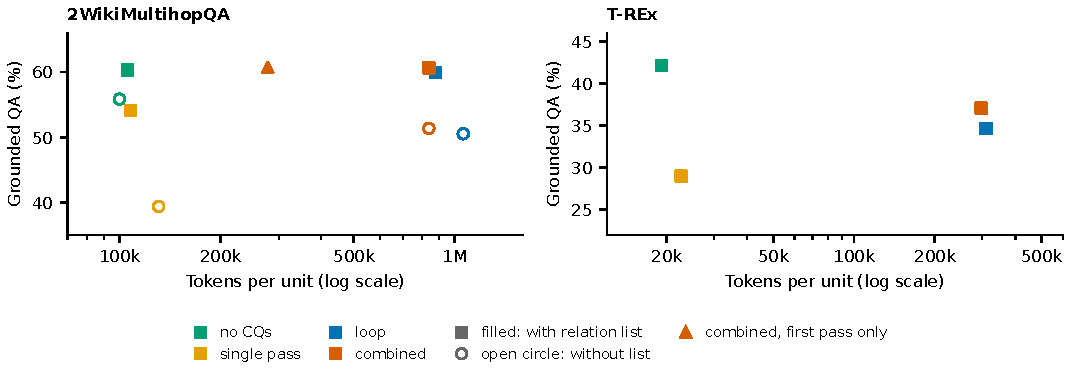
\includegraphics[width=\textwidth]{figures/fig_cost_quality_r64.pdf}
\caption{Seeded extraction without CQs was not distinguishable from the combined pipeline in grounded QA at a fraction of its tokens (106k against 838k per unit). Points are arm means of grounded QA against tokens per unit (log axis); intervals for the contrasts are in Tables~\ref{tab:glance} and~\ref{tab:itext}. Left, 2Wiki: arms with and without the list. Right, T-REx: seeded arms only. Qwen.}
\label{fig:costquality}
\end{figure*}}{}

The Exp7 arms on T-REx, every arm given the original 22 names, repeat the comparison on a second corpus. Seeded extraction scored .421 grounded QA against .371 for the combined pipeline, 5.0 points higher (registered 90\% interval [1.1, 8.1]), at 19.1k tokens per unit against 298k. Seeded extraction led, so the registered equivalence test at $\pm$3 points did not establish equivalence there.

\paragraph{Three public extractors in the same setup.}
None of the three public extractors received a relation list, and each ran with released defaults. Unseeded extraction, which also had no list, scored .558 grounded QA on the same units (Table~\ref{tab:exp8}). Run with Qwen on 2Wiki in the Exp7 setup (60 units, none failed), iText2KG wrote 1,899 facts, more than any arm in Table~\ref{tab:exp8}, and reached .430 grounded QA (Table~\ref{tab:itext}). That is 17.3 points below seeded extraction and 17.6 below the combined pipeline (both descriptive), at 478.8k tokens per unit against 105.9k and 837.7k. Against the single pass it was 3.7 points higher in grounded QA (interval includes zero) and 11.6 in answer correctness.
EDC, a second public extractor, induces its schema from the text and canonicalises it itself, and we ran it on the same model and engine with its released defaults (Self Canonicalization)~\cite{zhang2024edc}. It scored .445 grounded QA and .629 answer correctness (Table~\ref{tab:itext}), 5.1 points ([0.5, 10.0]) and 19.6 points ([14.8, 24.7]) above the single pass. EDC scored 15.8 points below seeded extraction in grounded QA ([$-$19.3, $-$12.3]; answer correctness $-$4.9 [$-$7.7, $-$2.5]), at 618.4k tokens per unit against 105.9k, and 16.1 points below the combined pipeline ([$-$20.1, $-$12.4]). EDC was also given the same 22-name list as its target schema, with the names as definitions (its Target Alignment mode), on the 30 units of one run seed; these arm means are on 30 units, so they differ from the 60-unit table values. It scored .458 grounded QA (.613 answer correctness) with the list against .454 (.633) without it, +0.4 points ([$-$2.7, 2.9], registered: not established), with 824 against 1,356 facts per unit. Seeded extraction scored 14.6 points above EDC with the list ([10.4, 18.5], registered: improved, Holm $p$ = 0.0003), so giving EDC the same list did not close the gap. All other differences involving EDC are descriptive.

AutoSchemaKG, a third public extractor, also induces its schema from the text~\cite{bai2026autoschemakg}. We ran it with its released defaults on the same model family, chunks, answerer and scorer, on 30 2Wiki shards with one run seed, and report the comparison as descriptive. Its entity-relation triples, the variant comparable to the other arms, scored .213 grounded QA and .446 answer correctness with 1,256.6 facts at 1,557.8k tokens per unit (Table~\ref{tab:itext}). On the same 30 shards, the stored seeded extraction scored .604 and .679, the combined pipeline .631 and .677, and the single pass .404 and .425. It scored 39.2 points below seeded extraction in grounded QA ([$-$44.0, $-$34.4]; answer correctness $-$23.3 [$-$27.5, $-$20.0]), and 41.9 points below the combined pipeline ([$-$46.3, $-$38.3]; $-$23.1 [$-$27.3, $-$19.0]). Against the single pass it scored 19.2 points lower in grounded QA ([$-$26.0, $-$13.1]), and the answer correctness difference was +2.1 ([$-$5.0, 9.4]; the interval includes zero).

Requiring a matching relation class changed each arm's grounded QA by at most 1.2 points and left the gaps unchanged or wider (post hoc reanalysis of the stored predictions). As a descriptive observation, the gold evidence pairs reached the 60 retrieved facts in 88.5\% of cases for seeded extraction, 81.0\% for iText2KG, 75.6\% for EDC and 57.7\% for AutoSchemaKG triples. Relaxing entity linking changed these reach rates by at most 0.5 points in every arm (post hoc, stored graphs).

\begin{table*}[t]
\centering
\caption{Three public extractors against Exp7 arms (Qwen, 2Wiki, 60 shard $\times$ run seed units; descriptive). EDC ran with its released defaults (Self Canonicalization). The AutoSchemaKG rows cover 30 shards with one run seed, and their differences are taken against the stored arms on those shards. AutoSchemaKG's entity-relation triples are the comparable variant; its full graph also holds concept and event edges. Tokens are per unit, in thousands. The difference rows give each extractor minus the arm, in points, with 95\% intervals.}
\label{tab:itext}
\footnotesize\setlength{\tabcolsep}{3pt}
\begin{tabular}{lcccc}
\toprule
 & Grounded QA & Answer correctness & Facts & Tokens (k) \\
\midrule
iText2KG & .430 [.393, .470] & .549 [.503, .596] & 1,899 & 478.8 \\
EDC & .445 [.398, .493] & .629 [.583, .676] & 1,357.7 & 618.4 \\
AutoSchemaKG, entity-relation triples & .213 [.175, .252] & .446 [.396, .490] & 1,256.6 & 1,557.8 \\
AutoSchemaKG, full graph & .096 [.073, .121] & .233 [.200, .260] & 18,360 & 1,557.8 \\
Seeded extraction & .603 & .678 & 1,472 & 105.9 \\
Combined & .606 & .655 & 1,435 & 837.7 \\
Single pass (L0) & .394 & .433 & 725 & 131.0 \\
\midrule
iText2KG $-$ seeded extraction & $-$17.3 [$-$21.0, $-$13.9] & $-$12.9 [$-$16.3, $-$10.0] & & \\
iText2KG $-$ combined & $-$17.6 [$-$20.8, $-$14.1] & $-$10.6 [$-$14.1, $-$7.5] & & \\
iText2KG $-$ single pass & $+$3.7 [$-$1.5, 9.3] & $+$11.6 [5.6, 18.2] & & \\
EDC $-$ seeded extraction & $-$15.8 [$-$19.3, $-$12.3] & $-$4.9 [$-$7.7, $-$2.5] & & \\
EDC $-$ combined & $-$16.1 [$-$20.1, $-$12.4] & $-$2.6 [$-$5.9, 0.5] & & \\
EDC $-$ single pass & $+$5.1 [0.5, 10.0] & $+$19.6 [14.8, 24.7] & & \\
AutoSchemaKG triples $-$ seeded extraction & $-$39.2 [$-$44.0, $-$34.4] & $-$23.3 [$-$27.5, $-$20.0] & & \\
AutoSchemaKG triples $-$ combined & $-$41.9 [$-$46.3, $-$38.3] & $-$23.1 [$-$27.3, $-$19.0] & & \\
AutoSchemaKG triples $-$ single pass & $-$19.2 [$-$26.0, $-$13.1] & $+$2.1 [$-$5.0, 9.4] & & \\
\bottomrule
\end{tabular}
\end{table*}

\paragraph{Retrieval over the same chunks.}
On the same 2Wiki units, seeded extraction reached .669 answer correctness in a rerun on the retrieval arms' own serving engine (.678 in the stored run, Table~\ref{tab:itext}). Retrieval-augmented generation from the top 5 chunks reached .515, and .500 with the 22-name list as a hint. Answer correctness is the common measure because the retrieval arms have no graph facts, so grounded QA cannot be computed for them. With no context, the answer model reached .325 from its own knowledge (descriptive); seeded extraction scored 35.3 points higher ([30.1, 40.1]). The graph scored 15.4 points above chunk retrieval ([10.6, 19.8]) and 16.9 above list-hinted retrieval ([11.1, 22.3]), and both comparisons were registered as improved.

The grounded-QA results above use graph facts only. When passages were added to the retrieved facts (hybrid QA) and the graph facts were capped at 60, every pipeline scored above vector-only QA (.502): LOOP+seed .725, L0+seed .716, U-ext+seed .709, Combined .699 and L0 .626 (60 units). Raising the fact cap from 30 to 60 raised U-ext+seed by 12.4 points ([9.3, 15.3]) and Combined by 9.6 ([7.2, 11.7]); both were registered as improved in answer correctness. In the stored run with up to 30 facts the scores were L0+seed .692, LOOP+seed .671, Combined .603, L0 .600 and U-ext+seed .585 (Appendix Table~\ref{tab:newchecks}): with 30 facts the arms with the most facts ranked lowest, and with 60 the four list or full-extraction arms were close. The cap was the setting we varied.

\section{What CQs Add: Each Fact Counts}
\label{sec:res-cqs}
\label{sec:res-coverage}

Two results on the equal-fact-count check come first. With the relation list, the guided single pass scored 39.1 points above an equal-size random subset of seeded extraction in grounded QA ([34.2, 44.1]); a registered test asked whether the random subset scores higher, and it did not. The lead held against further selectors, among them selections made with the CQs or balanced over chunks (below). Without the list the relation-frequency selection scored 8.0 points above the guided pass ([2.7, 13.3]; registered), and on T-REx without the list the contrast with a random subset was not established (6.6 points, [$-$5.8, 12.2]).

Without the list, U-ext raised grounded QA over L0 by 16.5 points ([10.6, 21.7], post hoc) by writing 1,704 facts against 725. The check compares the CQ-guided facts with facts chosen at random: we drew a uniform random subset of the stored U-ext graph (or of the listed graph, for the listed comparison) down to the fact count of the matching single pass, and the same answerer and scorer scored it. The plan was fixed before any model call. Without the list, the single pass scored 28.2 points above an equal-size random subset of open extraction ([23.4, 33.2]). On T-REx with the list, the single pass scored 7.4 points above an equal-size random subset of seeded extraction ([2.9, 12.8], Holm $p$ = 0.001, registered: improved). Two heuristic selections, one by relation frequency and one by entity centrality, cut the extraction graph to the guided graph's fact count. With the list, the CQ-guided single pass stayed ahead of both, by 16.6 points against the relation-frequency selection ([11.4, 22.1]) and 25.8 against the centrality selection ([20.5, 30.5]) in grounded QA (registered; Appendix Table~\ref{tab:selection}).

On 2Wiki with the list (60 units), the guided pass scored 25.0 points above the chain-preserving selector ([19.8, 30.1]) and 14.3 above the model selector ([8.9, 19.3]) in grounded QA (both registered: improved, Holm $p$ = 0.0002; Appendix Table~\ref{tab:selection}). Selections by the CQs of the unit and balanced over chunks scored below the guided pass by 33.3 points ([28.3, 37.7]) and 37.2 points ([31.6, 41.4]) in grounded QA (both registered: improved, Holm $p$ = 0.0004 and 0.0005). This separates CQ-guided extraction from CQ-guided selection.

CQs also leave a schema that answers structured queries. On 40 fresh CQs per shard and run seed, written from random chunks with a neutral prompt, the combined pipeline passed 13.5 points more through SPARQL than seeded extraction ([10.7, 16.3]).

\section{Discussion}
\label{sec:discussion}

\paragraph{A relation list lifts extraction.}
The relation list raised grounded QA in every Exp7 pipeline on 2Wiki. Neither gold relations nor the exact names were needed, since synonyms, a corpus-induced list and lists induced outside the evaluation shards raised the single pass on both corpora (Section~\ref{sec:res-schema}). The full list and the induced lists, which cover most gold relations, raised every pipeline.

\paragraph{Seeded extraction against the combined pipeline and the public extractors.}
Seeded extraction matched the combined pipeline in grounded QA (Section~\ref{sec:res-cost}), and its fact precision passed the non-inferiority test (.925 against .716). The public extractors received no relation list, except in one run with the list (Section~\ref{sec:res-cost}). iText2KG wrote the most facts of any arm yet scored below seeded extraction (Table~\ref{tab:itext}), so writing more facts did not by itself deliver that score. On 2Wiki the listed graph answered more questions correctly than retrieval over the same chunks, while the list given to retrieval as a hint did not raise answer correctness.

\paragraph{At a fixed fact count, CQ-guided facts scored higher.}
At equal fact count and with the relation list, the CQ-guided single pass scored above a uniform random subset of seeded extraction, on the multi-hop corpus (Section~\ref{sec:res-cqs}) and on T-REx. It also scored above two heuristic subsets of the same graph at the same fact count, one keeping the facts of the most frequent relations and one the facts whose end entities are most central, and above a chain-preserving and a model-scored selector (Appendix Table~\ref{tab:selection}).

\section{Conclusion}
\label{sec:conclusion}

In this pipeline, how well a graph answered held-out questions followed what reached it. A relation list induced from the corpus, without gold relations, raised answer correctness by 16.3 points on 2WikiMultihopQA and 12.5 on T-REx, and lists induced only outside the evaluation documents also raised grounded QA on both corpora. On the multi-hop corpus, once the extractor had a relation list, extraction without CQs was not distinguishable from the combined pipeline in grounded QA (0.3 points) with fewer tokens than the combined pipeline's first pass alone, and scored 15.8 to 39.2 points above three public extractors. At equal fact count, the CQ-guided single pass scored above a random subset of the listed extraction, and it also scored above heuristic, chain-preserving and model-scored selections, and above selections made with the CQs or balanced over chunks. In these corpora, giving the extractor a relation list and extracting from every chunk reached the combined pipeline's grounded QA with fewer tokens; with the list and a fixed fact count, CQ-guided extraction kept more answerable facts than random and question-agnostic subsets.


\bibliographystyle{IEEEtran}
\bibliography{references}

\appendices
\renewcommand{\arraystretch}{0.88}
\section{Additional Results and Records}
\label{app:experiments}

\begin{table*}[!t]
\centering
\caption{Results at a glance. Values are differences in points unless marked; $n$ is the number of shards (two run seeds averaged within a shard where used). Status is the contrast's standing in the plan. A dash means the contrast was not repeated. For the equal-fact-count rows, the registered test asks whether the selection scores above the guided pass, and the status reports that it did not.}
\label{tab:glance}
\scriptsize\setlength{\tabcolsep}{2pt}
\begin{tabular}{P{3.7cm}P{0.9cm}P{1.4cm}P{3.0cm}P{6.0cm}P{0.6cm}P{2.3cm}}
\toprule
Claim & Exp & Model, corpus & Contrast & Value [95\% interval] & $n$ & Status \\
\midrule
The list raises grounded QA & Exp7 & Qwen, 2Wiki & With vs.\ without list, four pipelines & L0 +14.7 [10.9, 18.4]; LOOP +9.4 [6.4, 12.2]; combined +9.3 [6.0, 12.1]; U-ext +4.5 [0.7, 8.8] & 30 & Descriptive (intervals only) \\
Synonym list, answer correctness & Exp7 & Qwen, 2Wiki & Synonym list $-$ no list & L0 +15.4 [11.3, 19.5]; U-ext +1.6 [$-$1.4, 4.2] & 30 & Registered: improved (L0); not established (U-ext) \\
Equal fact count: guided single pass above random subset of U-ext & Exp7 & Qwen, 2Wiki & L0 $-$ random subset of U-ext at L0's fact count; with seed, L0+seed $-$ random subset of U-ext+seed, QA & +28.2 [23.4, 33.2]; +39.1 [34.2, 44.1] & 30 & Registered: random subset not above the guided pass (both) \\
Expansion raises grounded QA & Exp4, Exp5 & Qwen, 2Wiki & G $-$ L0 & +9.1 [4.7, 13.8]; +9.6 [5.2, 14.8] & 40; 24 & Post hoc secondary \\
Iteration did not separate from one batch of the same CQs & Exp2 & Qwen, 2Wiki & Iteration $-$ one batch, recall & +1.2 [$-$3.5, 5.7], crossed shard $\times$ run seed interval & 24 & Registered primary (inconclusive) \\
Hybrid QA: no detectable change at 1$\times$, lower at 4$\times$ budget in Qwen on 2Wiki & Exp8 & as above & 160 vs.\ 40 CQs, 1$\times$ & $-$3.6 to +0.6, all intervals include 0 (Table~\ref{tab:exp9}). At 4$\times$ budget, Qwen 2Wiki $-$9.1 [$-$13.8, $-$5.5] & 20--33 & Registered primary \\
More CQs raise KG-only QA & Exp8 & Qwen, Gemma; 2Wiki, T-REx & 160 vs.\ 40 CQs, 1$\times$ & +3.5 to +10.9, all intervals above 0 (Table~\ref{tab:exp9}) & 20--33 & Secondary measure \\
Guided repair not improved over random & Exp4, Exp5 & Qwen, 2Wiki & Guided $-$ random patches, QA & +1.9 [$-$1.6, 5.3]; $-$0.3, one-sided upper bound 3.1 & 40; 24 & Exp5 primary, margin 5; Exp4 inconclusive \\
Combined pipeline leads loop on uncapped recall and recall at equal fact counts, trails on capped recall & Exp7 & Qwen, 2Wiki & Combined $-$ LOOP+seed, recall & Uncapped +5.6 [4.2, 7.0]; capped $-$8.7 [$-$10.6, $-$6.8]; equal fact counts +1.1 [0.5, 1.9] & 30 & Registered primary (uncapped); matching in plan \\
Seeded extraction without CQs was not distinguishable from the combined pipeline & Exp7 & Qwen, 2Wiki & Combined $-$ U-ext+seed, QA & +0.3 [$-$3.1, 3.5]; 106k against 838k tokens per unit; answer correctness, seeded extraction higher by 2.3 [$-$0.2, 4.4] (post hoc) & 30 & Added arm \\
Combined pipeline passes more fresh CQs than seeded extraction without CQs & Exp7 & Qwen, 2Wiki & Combined $-$ U-ext+seed, fresh-CQ pass rate & +13.5 [10.7, 16.3]; LLM judge of the builder's family & 30 & Secondary, in the Exp7 plan; added arm \\
Most inexact gold facts are omissions & Exp6 & Qwen, 2Wiki & Omission share of inexact gold facts & 87.3\% of 1,336 & --- & Analysis of Exp2 graphs \\
\bottomrule
\end{tabular}
\end{table*}

\begin{table*}[!ht]
\centering
\caption{Exp8, other arms against the reference of 40 CQs at 1$\times$, in points. The arms with 160 CQs have shard-cluster BCa 95\% intervals; the 40-CQ arm at 4$\times$ is an arm-mean difference with no registered interval. Tokens are the mean ratio of 160 CQs at 4$\times$ to the reference.}
\label{tab:exp9other}
\scriptsize\setlength{\tabcolsep}{2.5pt}
\begin{tabular}{p{4.1cm}cccc}
\toprule
 & Qwen, T-REx & Gemma, T-REx & Gemma, 2Wiki & Qwen, 2Wiki \\
\midrule
KG-only QA, 160 CQs, 4$\times$ & +4.7 [1.6, 8.0] & +5.0 [1.7, 8.2] & +10.6 [2.5, 17.2] & +1.6 [$-$4.7, 5.7] \\
KG-only QA, 40 CQs, 4$\times$ (mean) & +1.5 & $-$0.5 & +1.0 & 0.0 \\
Evidence recall, 160 CQs, 4$\times$ & +1.9 [0.8, 3.9] & +0.6 [$-$0.2, 2.0] & +9.5 [5.9, 15.6] & +12.0 [8.8, 15.6] \\
Hybrid QA, 160 CQs, 4$\times$ & +0.9 [$-$2.8, 4.2] & +0.3 [$-$2.2, 2.6] & $-$0.9 [$-$4.7, 3.4] & $-$9.1 [$-$13.8, $-$5.5] \\
Precision, 160 CQs, 4$\times$ & $-$12.4 [$-$18.0, $-$7.8] & $-$1.2 [$-$4.8, 2.4] & +3.3 [$-$0.6, 7.1] & $-$12.2 [$-$17.0, $-$6.4] \\
Precision, 160 CQs, 1$\times$ & 0.0 [$-$5.2, 5.0] & $-$0.5 [$-$5.2, 3.8] & +4.9 [0.8, 9.4] & $-$4.0 [$-$9.0, 0.7] \\
Tokens, 160 CQs 4$\times$ / reference & 2.8 & 1.9 & 3.8 & 4.0 \\
\bottomrule
\end{tabular}
\end{table*}

\begin{table*}[!t]
\centering
\caption{Exp8: 160 CQs at the 1$\times$ token budget against the reference of 40 CQs at 1$\times$. Differences in points with shard-cluster BCa 95\% intervals; $n$ is the number of shards in the contrast. Post hoc 90\% intervals for hybrid QA, left to right: [$-$1.8, 2.3], [$-$1.7, 3.1], [$-$3.4, 4.7] and [$-$8.1, 0.3].}
\label{tab:exp9}
\footnotesize\setlength{\tabcolsep}{3.5pt}
\begin{tabular}{lcccc}
\toprule
 & Qwen, T-REx & Gemma, T-REx & Gemma, 2Wiki & Qwen, 2Wiki \\
 & ($n$=33) & ($n$=26) & ($n$=20) & ($n$=24) \\
\midrule
Hybrid QA & +0.3 [$-$2.2, 2.6] & +0.6 [$-$2.2, 3.6] & +0.6 [$-$3.7, 5.6] & $-$3.6 [$-$8.9, 1.0] \\
KG-only QA & +3.5 [0.7, 6.8] & +5.6 [2.0, 9.8] & +10.9 [4.1, 15.9] & +6.2 [0.3, 10.4] \\
Evidence recall (uncapped) & +0.3 [$-$1.1, 2.1] & +1.0 [0.1, 2.3] & +9.2 [5.5, 15.4] & +9.9 [6.9, 13.2] \\
\bottomrule
\end{tabular}
\end{table*}

\begin{table*}[!ht]
\centering
\caption{Original Qwen runs and the Gemma replication, in points with 95\% intervals ($n$ in shards or units). Labels are the plans' decision labels; for Exp5 the margin is 5 points. A dash means no value or no run. Nemotron is a third model whose grounded QA stayed at floor (at most .047 in every arm, post hoc).}
\label{tab:replication}
\scriptsize\setlength{\tabcolsep}{3pt}
\begin{tabular}{P{3.7cm}P{3.7cm}P{4.2cm}P{3.5cm}}
\toprule
Experiment and contrast & Qwen & Gemma & Nemotron \\
\midrule
Exp1, iteration over none (by construction, plan) & +21.4 [16.2, 27.1] & +42.1 [33.6, 50.7] & invalid or at floor \\
Exp4, GR over L0 & +9.7 [4.1, 15.0] & +13.1 [7.8, 18.4] & invalid or at floor \\
Exp5, evaluation-guided over random repair & $-$0.3, upper bound 3.1 (one-sided), not improved & +1.5 [$-$3.1, 6.5], not improved & $-$0.7 [$-$1.9, 0.0] \\
Exp7, recall, combined over LOOP+seed & +5.6 [4.2, 7.0] & +9.2 [7.6, 11.4] ($n$=60) & +13.1 [8.9, 16.8] ($n$=41) \\
Exp7, recall, combined over L0+seed & +14.0 [12.1, 15.9] & +10.2 [2.1, 16.1] & +16.7 [11.8, 20.9] \\
Exp7 design on T-REx, combined $-$ LOOP+seed & --- & +1.6 [$-$0.9, 4.4], not established ($n$=27) & +1.2 [$-$0.6, 4.1], not established ($n$=12) \\
Exp7 design on T-REx, combined $-$ L0+seed & --- & +2.7 [$-$0.4, 5.8], not established & --- \\
\bottomrule
\end{tabular}
\end{table*}

\begin{table*}[!ht]
\centering
\caption{Checks added after the main study, Qwen. Hybrid QA with up to 30 graph facts against vector-only QA (.502 [.460, .544]) and fact precision judged by Gemma, both on the 2Wiki Exp7 graphs (points, 95\% intervals, 30 shards); grounded QA, class-aligned recall and tokens per unit (thousands) for the Exp7 arms on T-REx (33 shards, one run seed). Precision was not measured for L0.}
\label{tab:newchecks}
\scriptsize\setlength{\tabcolsep}{2.5pt}
\begin{tabular}{lcccccc}
\toprule
 & Hybrid QA & Hybrid $-$ vector & Precision & QA, T-REx & Recall, T-REx & Tokens (k) \\
\midrule
L0 & .600 & +9.8 [4.3, 14.6] & --- & --- & --- & --- \\
L0+seed & .692 & +19.0 [14.7, 22.5] & .874 [.856, .890] & .290 & .173 & 22.7 \\
LOOP+seed & .671 & +16.9 [12.2, 21.0] & .802 [.785, .819] & .346 & .189 & 310 \\
Combined & .603 & +10.1 [5.3, 14.2] & .716 [.686, .741] & .371 & .228 & 298 \\
U-ext+seed & .585 & +8.3 [2.2, 13.9] & .925 [.913, .938] & .421 & .184 & 19.1 \\
\bottomrule
\end{tabular}
\end{table*}

\subsection{Further relation-list checks}
\label{app:seednames}
\paragraph{Relation list names.} Table~\ref{tab:seednames} lists the 22 names of each 2Wiki list, copied from the list files, in alphabetical order.

\begin{table}[t]
\centering
\caption{The original list (relation names taken from the 2WikiMultihopQA training split) the induced list (proposed by an LLM from 300 corpus chunks), and a list induced the same way from 300 chunks outside the evaluation shards.}
\label{tab:seednames}
\scriptsize\setlength{\tabcolsep}{3pt}
\begin{tabular}{lP{6.6cm}}
\toprule
Original & award received, cause of death, child, composer, country, country of citizenship, country of origin, date of birth, date of death, director, educated at, father, founded by, inception, mother, occupation, performer, place of birth, place of burial, place of death, publication date, spouse \\
Induced & award, based on, birth date, birth place, cast member, child, country, death date, death place, director, employer, genre, located in, member of, nationality, occupation, parent, position held, release year, sibling, spouse, title \\
Induced outside shards & based on, birth date, birth place, cast member, child, death date, death place, director, employer, genre, location, member of, nationality, occupation, parent, producer, publication date, release year, sibling, spouse, title, writer \\
\bottomrule
\end{tabular}
\end{table}

\paragraph{Synonyms and alignment.}
Class-aligned recall fell under synonyms, as name alignment predicts. In U-ext the synonym list's answer correctness was $-$1.5 points against the original list ([$-$4.2, 1.4]). A post hoc re-analysis of stored predictions tests the original list's gain without name matching (Table~\ref{tab:seedalign}). For the three pipelines that use CQs the effect stays above zero on both measures, and class-free recall keeps 65 to 85\% of the class-aligned effect.

\begin{table}[!htb]
\centering
\caption{Post hoc list effect in points (95\% BCa intervals, 30 shards), Exp7. Class-free recall ignores relation classes when matching triples to gold; answer correctness drops the grounding requirement.}
\label{tab:seedalign}
\scriptsize\setlength{\tabcolsep}{2.5pt}
\begin{tabular}{lccc}
\toprule
 & Recall, class aligned & Class-free recall & Answer correct \\
\midrule
L0 & +11.4 [9.3, 14.5] & +9.7 [7.6, 12.9] & +13.8 [10.5, 17.2] \\
LOOP & +7.7 [5.4, 9.7] & +5.0 [2.9, 6.9] & +7.9 [4.8, 10.7] \\
Combined & +10.3 [8.0, 12.6] & +6.8 [5.1, 8.6] & +7.0 [4.0, 9.7] \\
U-ext & +2.1 [1.0, 3.5] & +0.6 [$-$0.7, 2.3] & +3.0 [0.0, 6.6] \\
\bottomrule
\end{tabular}
\end{table}

\subsection{Seeded extraction against the combined pipeline}
A post hoc 90\% interval of [$-$2.6, 3.0] around the difference in grounded QA (Section~\ref{sec:res-cost}) excludes differences beyond about 3 points in either direction. On T-REx the combined pipeline found more gold evidence (class-aligned recall +4.4, 90\% [3.0, 6.0]).

\subsection{Fact-count check and coverage}
With the list, U-ext raised grounded QA over L0+seed by 6.3 points ([2.6, 9.4], post hoc).

\paragraph{Heuristic selections at equal fact count.} Appendix Table~\ref{tab:selection} gives the eight registered contrasts of the equal-fact-count check against the CQ-guided pass.

\begin{table}[!htb]
\centering
\caption{Guided single pass minus a selection of the extraction graph at the guided pass's fact count (Qwen on 2Wiki, 60 shard $\times$ run seed units; grounded QA, differences in points with 95\% intervals). Status gives the outcome of the registered test of whether the selection scores above the guided pass. The selectors read no questions or gold relations; one arm reads the unit's CQs.}
\label{tab:selection}
\scriptsize\setlength{\tabcolsep}{3pt}
\begin{tabular}{llcl}
\toprule
Selection & Relation list & Guided $-$ selection & Status \\
\midrule
Entity centrality & none & +14.4 [9.5, 19.5] & Reg.: guided higher \\
Relation frequency & none & $-$8.0 [$-$13.3, $-$2.7] & Reg.: selection higher \\
Entity centrality & seeded & +25.8 [20.5, 30.5] & Reg.: guided higher \\
Relation frequency & seeded & +16.6 [11.4, 22.1] & Reg.: guided higher \\
Chain-preserving & seeded & +25.0 [19.8, 30.1] & Reg.: guided higher \\
Model-scored & seeded & +14.3 [8.9, 19.3] & Reg.: guided higher \\
CQ-selected & seeded & +33.3 [28.3, 37.7] & Reg.: guided higher \\
Chunk-balanced & seeded & +37.2 [31.6, 41.4] & Reg.: guided higher \\
\bottomrule
\end{tabular}
\end{table}

\subsection{Hybrid QA and CQ count}
\label{sec:res-hybrid}
Table~\ref{tab:exp9other} gives the CQ-count settings. On the Exp7 graphs (Qwen, 2Wiki), hybrid QA scored above vector-only QA (.502 [.460, .544]) in every pipeline (Table~\ref{tab:newchecks}); the run with 60 graph facts is reported in Section~\ref{sec:res-cost}. In Exp8, four times as many CQs at the same budget raised KG-only QA in all four settings (Table~\ref{tab:exp9}); hybrid QA, the registered primary measure, did not separate from the 40-CQ reference.


\subsection{Evaluation-guided repair}
\label{sec:res-loop}
Iterative CQ generation in Exp2 grew the CQ set from 12.0 to 85.8 per shard and evidence recall from .093 to .377 (Table~\ref{tab:glance}). Evaluation-chosen patches scored 1.9 points above random patches ([$-$1.6, 5.3]). Exp5 repaired queries first and patched only graph-side failures, gating each patch on reserved curation CQs and never on held-out questions; evaluation-chosen patches again did not improve on random patches ($-$0.3; upper bound 3.1, margin 5).

\subsection{Combined pipeline versus the loop}
In Exp7 the combined pipeline and LOOP+seed (Table~\ref{tab:exp8}) used 838k and 878k tokens in Qwen. Without a per-question triple cap the combined pipeline led in all three models, and at equal fact counts the lead shrank to 0.3 to 1.1 points (Table~\ref{tab:equalcount}). In Qwen, capped recall favoured the loop (Table~\ref{tab:glance}). On T-REx with Gemma, neither registered contrast was established (Table~\ref{tab:replication}).

\begin{table}[!htb]
\centering
\caption{Exp7: recall lead of the combined pipeline over LOOP+seed, in points with 95\% intervals; uncapped means without a per-question triple cap. Intervals resample shard $\times$ run seed units by shard.}
\label{tab:equalcount}
\scriptsize\setlength{\tabcolsep}{2.5pt}
\begin{tabular}{lccc}
\toprule
Model & Units & Uncapped recall lead & At equal fact counts \\
\midrule
Qwen & 60 & +5.6 [4.2, 7.0] & +1.1 [0.5, 1.9] \\
Gemma & 60 & +9.2 [7.6, 11.4] & +0.3 [$-$0.6, 1.1] \\
Nemotron & 41 & +13.1 [8.9, 16.8] & +0.3 [$-$0.5, 1.3] \\
\bottomrule
\end{tabular}
\end{table}

\subsection{Further checks}
Of the 2,196 gold evidence facts in the Exp2 graphs, 860 were reproduced exactly, 74 had a wrong value, 96 were split across entities and 1,166 were missing. Omissions made up 87.3\% of the 1,336 inexact facts. SHACL shapes~\cite{knublauch2017shacl} flagged 0.15\% of the inexact facts ([0, 0.37]) and 25.1\% of correct facts.

\paragraph{Exp3.} The fixed relation list scored higher than prompt optimisation with MIPROv2 or GEPA on 400 test questions, with and without matching the number of triples (Table~\ref{tab:exp3}, arm means).

\begin{table}[!htb]
\centering
\caption{Exp3 evidence recall on 400 test questions. The last column equalises the number of triples across arms.}
\label{tab:exp3}
\small\setlength{\tabcolsep}{3.5pt}
\begin{tabular}{lcc}
\toprule
 & Recall & Recall, equal triples \\
\midrule
Relation list & .425 & .411 \\
MIPROv2 & .363 & .255 \\
GEPA & .356 & .337 \\
Default prompt & --- & .181 \\
\bottomrule
\end{tabular}
\end{table}

\paragraph{Exp1.} Iterative CQ refinement raised the gold ASK-query pass rate over no refinement on building-ontology questions (+21.4 points, [16.2, 27.1], 35 test questions; positive by construction).




\begin{IEEEbiography}[{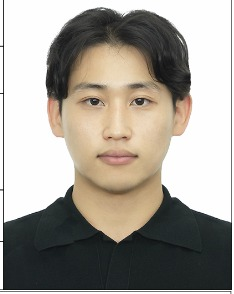
\includegraphics[width=1in,height=1.25in,clip,keepaspectratio]{figures/bio_minwoo_kim.jpg}}]{Minwoo Kim}
received the M.S. degree in data science and artificial intelligence from the Graduate School of AI$\cdot$SW, Sogang University, Seoul, Republic of Korea, in 2026. He is with the Manufacturing AX Research Laboratory at INTERX, Seoul, working on large language model (LLM) pipelines for industrial AI applications. His research emphasizes deterministic, auditable pipelines and empirical evaluation of knowledge graph construction and question answering systems. His broader interests include knowledge-graph engineering, autonomous manufacturing, agentic AI, and speech recognition.
\end{IEEEbiography}

\begin{IEEEbiography}[{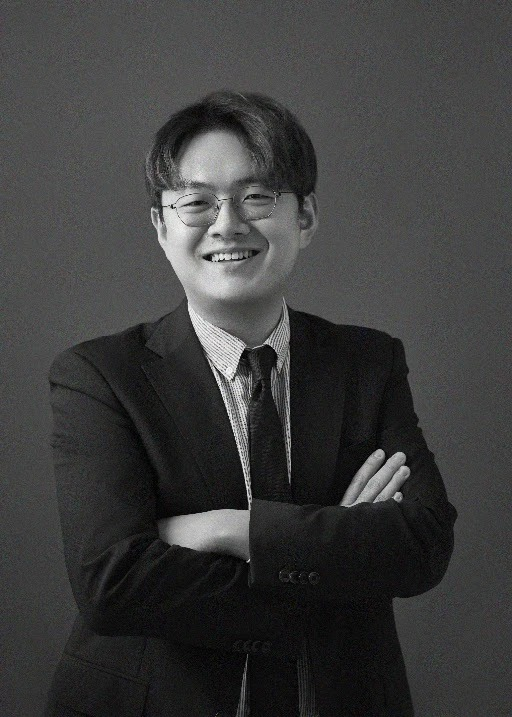
\includegraphics[width=1in,height=1.25in,clip,keepaspectratio]{figures/bio_hail_jung.jpg}}]{Hail Jung}
is currently an Assistant Professor with the Department of Industrial and Systems Engineering at Seoul National University of Science and Technology, Seoul, Republic of Korea. He is also a founding member and the Chief Technology Officer (CTO) of INTERX, a manufacturing AI solution provider. He has served as an ad-hoc referee for multiple academic journals, including the \emph{Journal of Business Research}.
\end{IEEEbiography}

\begin{IEEEbiography}[{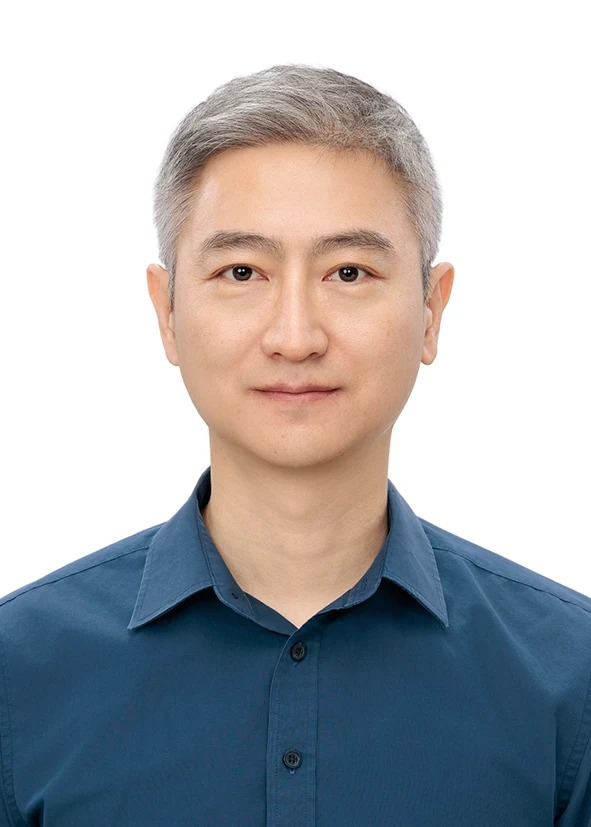
\includegraphics[width=1in,height=1.25in,clip,keepaspectratio]{figures/bio_hongdon_lee.jpg}}]{Hongdon Lee}
received the B.B.A. degree in business administration from Yonsei University, Seoul, Republic of Korea, in 2000, and the M.S. degree in statistics and data science from Korea National Open University, Seoul, in 2020. He is currently a Chief Researcher with INTERX, Seoul, Republic of Korea. His research interests include large language models (LLMs), vision-language models (VLMs), AI agents, and computer vision. He is an inventor on approximately ten patents related to generative AI for manufacturing innovation.
\end{IEEEbiography}

\end{document}
